\section{数据与信息}
我们生活的方方面面都离不开数据。数据析出了我们的生活轨迹,我们也在数据的指引下做出各种选择。\par
早上醒来,看一眼天气预服,发现今天的最低气温是-5\textdegree C,比昨天低了好多,看来要加衣服了;匆忙赶到教室,看了一眼时间,发现刚好是7:59,庆幸自己没有迟到;中午去超市购物,发现面包促销,全场打8折,就买了好多回去;睡前称一下体重,发现比上个月瘦了2斤,心中暗暗窃喜。像这样,温度、时间、价格、体重等等,都是具象的\textbf{数据(Data)}。\par
我们还可能遇到抽象的数据。学生的学号、员工的工号、公民身份证号,这些都是“编号”,它们比那些一眼就明白含义的数据要抽象,如果不加解释,我们就很难看懂,只会觉得那是一串无规律的数字。\par
有些数据的形式不太常规,比如一个人的姓名,它看上去又像数据,又不像数据——我们怎么能把汉字当成数字一样的东西呢?要解决这个困惑,我们可以给所有汉字进行\textbf{编码(Encoding)}。比如说,``赵钱孙李''分别定为``1, 2, 3, 4'',那么我们就可以把``赵''记为``1'',把``孙''记为``3''。像这样把所有汉字都编成表,接下来我们就可以用这张表来把汉字翻译成数字了。\par
\begin{table}[htbp]
\centering
\begin{tabular}{cccccccc}
\hline
\rule{0pt}{2.4ex}
\textbf{汉字} & \textbf{编码} & \textbf{汉字} & \textbf{编码} & \textbf{汉字} & \textbf{编码} & \textbf{汉字} & \textbf{编码}\\
\hline\hline
\rule{0pt}{2.4ex}
赵 & 1 & 钱 & 2 & 孙 & 3 & 李 & 4 \\
\hline
\rule{0pt}{2.4ex}
... & ... & ... & ... & ... & ... & ... & ... \\
\hline
\rule{0pt}{2.4ex}
何 & 21 & 吕 & 22 & 施 & 23 & 张 & 24 \\
\hline
\rule{0pt}{2.4ex}
... & ... & ... & ... & ... & ... & ... & ... \\
\hline
\rule{0pt}{2.4ex}
一 & 569 & 二 & 570 & 三 & 571 & 四 & 572 \\
\hline
\rule{0pt}{2.4ex}
... & ... & ... & ... & ... & ... & ... & ... \\
\hline
\end{tabular}
\caption{一个简单的汉字-数字编码表}
\end{table}
于是我们根据这个表,可以查出``张三''对应``24-571'',而``李四''对应``4-572''。这就是一个简单的编码过程。\par
同样的道理,我们如果拿到了``24-571'',就可以根据这张表查出``张三'';拿到了``4-572'',就可以根据这张表查出``李四''。这就是一个简单的\textbf{解码(Decoding)}过程。\par
地址也是数据,我们可以对地址进行编码。例如,中国邮政使用六位数字组成的邮政编码来划分邮件投递区域,比如说北京市是``10××××'',上海市是``20××××''。这样就可以用数据来指代我们想要表达的信息了。\par
还有更抽象的数据。一本电子书,一部电影,一款电子游戏,也是数据\footnote{广义地讲,实体书、绘画、雕塑等等也是数据。但这些已经远远超出了我们的讨论范围。}。在计算机中,它们都有相应的文件扩展名,像是\texttt{.epub}, \texttt{.mp4}, \texttt{.exe}之类。这些文件都以某种编码方式储存在计算机里,扩展名不同,说明它们的编码方式不同。如果要了解这些文件中的信息,就需要用正确的打开方式(比如使用支持\texttt{.epub}格式的电子书阅读器)才能对内容进行解码。\par
\subsection*{C++中的基本数据}
说了这么多,让我们回来看看C++中的数据吧。C++的数据可以分为两大类:\textbf{基本类型(Fundamental type)}和\textbf{复合类型(Compound type)}。本章删繁就简,只介绍三种基本的数据类型:整数、浮点数(小数),字符。\par
\subsubsection*{整数类型(Integer type)}
顾名思义,整型就是专为为表示整数而设计的类型。它不能表示小数。\par
C++为我们提供了很多内置的整数类型,我们可以直接使用。不同类型的区别主要在于以下两点:其一,有些可以表示负数,而有些不允许表示负数;其二,有些表示的数据范围较宽(我们可以把这个范围理解成``容量''),有些则较窄\footnote{容量是与内存空间有关的。如果某个类型占用的字节数为2,那么它只能表示$256^2=65536$个不同的整数。因此它无法表示十万以上的数据,我们需要用更宽的类型来表示。}。我们目前无需追究其中的细节,我会在第二章和后面的精讲篇中详细讨论这个问题。\par
\subsubsection*{浮点类型(Floating-point type)}
浮点类型有点像``科学记数法'',一个浮点数既有表示分数的部分(Fraction),又有表示冪次的部分(Exponent bias)。它既可以表示小数,也可以表示整数,并且数据范围非常宽\footnote{值得注意的是,浮点类型的数据都有精度限制,不能准确表示有效数字过多的数据。正因如此,浮点类型不适合用来表示和计算特别大的整数;这时应当使用整型。}。\par
C++同样提供了内置的浮点类型。不同类型的区别主要在于以下两点:其一,它们能表示的有效位数各不相同;其二,它们的冪指数范围有宽有窄。\par
\subsubsection*{字符类型(Character type)}
严格说来,字符型是一种特殊的整型。不同之处在于,字符数据不是用来``计算''而是用来``编码''的。\par
以最原始而最通用的ASCII码\footnote{美国信息标准交换代码(American Standard Code for Information Interchange, ASCII),是一套基于拉丁字母的编码系统,主要用于显示现代英语。}为例,它有若干控制字符和可显示字符,每个字符都有一个编码,如图1.1所示。读者无需记忆本图,只需知道它是一套编码系统即可。通过ASCII,每个拉丁字母都能编码成一个整数,比如字符\texttt{'0'}对应着编码48,字符\texttt{'A'}对应着编码65,字符\texttt{'a'}对应着编码97。\par
\begin{figure}[htbp]
    \centering
    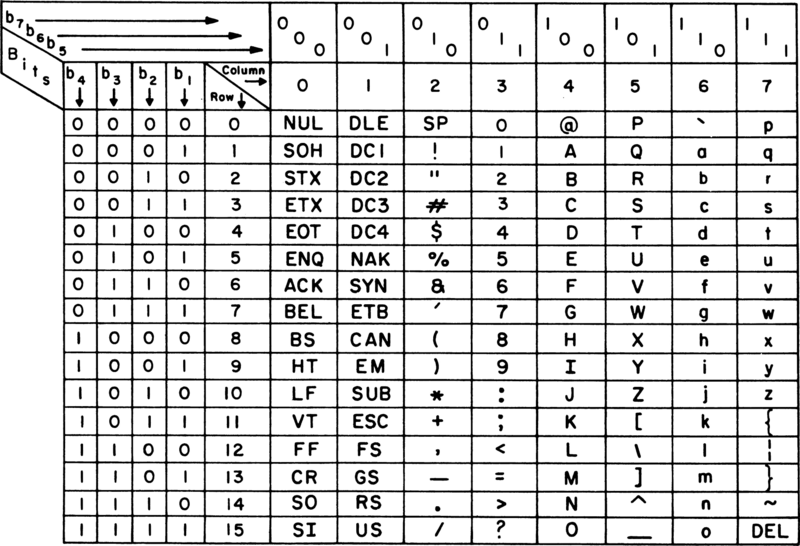
\includegraphics[width=0.75\textwidth]{../images/generalized_parts/01_ASCII.png}
    \caption{一个ASCII码表}
    \footnotesize{图片来源:维基共享资源}
\end{figure}
这套字符编码只适用于现代拉丁字母。如果要表示其它语言(比如中文)的字符,就需要用更复杂的编码规则。我们会在精讲篇中细细道来。\par
